% Figure from MATH 556 notes, section 33. Compile with the notes preamble.
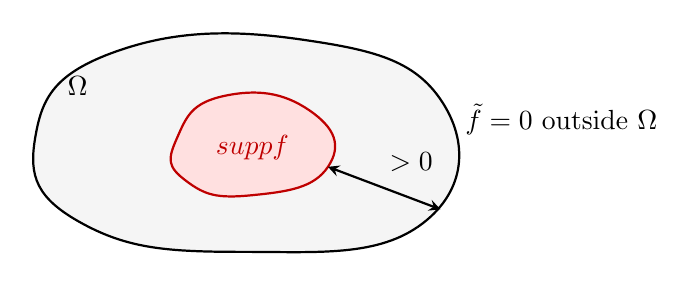
\begin{tikzpicture}[scale=1.2, >=stealth]
    \draw[thick, fill=gray!8] plot[smooth cycle, tension=0.8] coordinates {(-2.2,0.1) (-1.4,1.0) (0.6,1.15) (2.1,0.5) (1.9,-0.8) (0,-1.1) (-1.7,-0.8)};
    \node at (-1.75,0.65) {$\Omega$};
    \draw[thick, red!75!black, fill=red!12] plot[smooth cycle, tension=0.9] coordinates {(-0.7,0.1) (-0.2,0.55) (0.7,0.4) (0.9,-0.2) (0.1,-0.5) (-0.6,-0.35)};
    \node[red!75!black] at (0.1,0) {$\operatorname{supp} f$};
    \draw[<->, thick] (0.9,-0.2) -- (2.09,-0.65);
    \node[anchor=west] at (1.45,-0.15) {$> 0$};
    \node[anchor=west] at (2.25,0.3) {$\tilde f = 0$ outside $\Omega$};
\end{tikzpicture}
